% @Author: AnthonyKenny98
% @Date:   2020-04-08 10:23:56
% @Last Modified by:   AnthonyKenny98
% @Last Modified time: 2020-04-10 15:09:02
\begin{figure}[H]
\begin{centering}
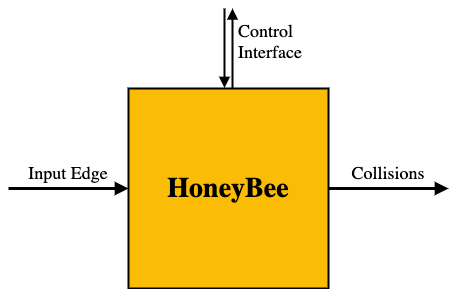
\includegraphics[width=0.6\linewidth]{chapters/chapter3/img/honeybee_interface_simple.png}
\mycaption{General Overview of HoneyBee Interface}{. The functional unit takes an edge $e$, defined by two points $p_1$ and $p_2$, as an input, and outputs a series of collisions. These collisions describe which grids an edge intersects. Its control interface allows for communication with a processor's main control unit.}
\label{fig:honeybee_interface_simple}
\end{centering}
\end{figure}